Il sito è strutturato nel seguente modo, partendo dall'alto e scendendo verso il basso:
	\begin{itemize}
		\item \textbf{Menu orrizontale con barra di ricerca}: sulla parte sinistra vi è un menu a schede, non appartenente al sito della facoltà di informatica ma all'ateneo UniBa. A prima lettura questo non è chiaro e può creare ambiguità. Inoltre un altro errore consiste nel fatto che non viene sfruttato al meglio l'angolo in alto a sinistra (punto di entrata dell'occhio dell'utente), dove sarebbe opportuno mettere il logo della facoltà. Per quanto riguarda la posizione della barra di ricerca, sulla destra, è buona. Le funzionalità della barra di ricerca verranno analizzate in una sezione dedicata sucessiva.
\begin{center}
\begin{figure}[h!]
           \begin{center}
           
\includegraphics[scale=0.40]{C:/Users/elepo/Desktop/UNI/WIM/ANALISI_SITO/Relazione/sez/Analisi/1.png}
           \caption{Menu orrizontale con barra di ricerca}
           \end{center}
  \end{figure}
\end{center}
		\item \textbf{Header}: contiene il logo della facoltà e la sua dicitura;
		\begin{center}
\begin{figure}[h!]
           \begin{center}
           
\includegraphics[scale=0.40]{C:/Users/elepo/Desktop/UNI/WIM/ANALISI_SITO/Relazione/sez/Analisi/2.png}
           \caption{Header}
           \end{center}
  \end{figure}
\end{center}
		\item \textbf{Pagina principale}: strutturata nel seguente modo:
			\begin{itemize}
				\item Parte sinistra: dedicata alle sezioni di seguito analizzate nelle sezioni di strutturazione dei contenuti, contatto con i social (facebook e twitter), login dell'area riservata del personale del dipartimento, una sezione riguardante la fatturazione elettronica (di cui personalmente non ho compreso il significato):
\begin{figure}[!htb]
   \begin{minipage}{0.48\textwidth}
     \centering
     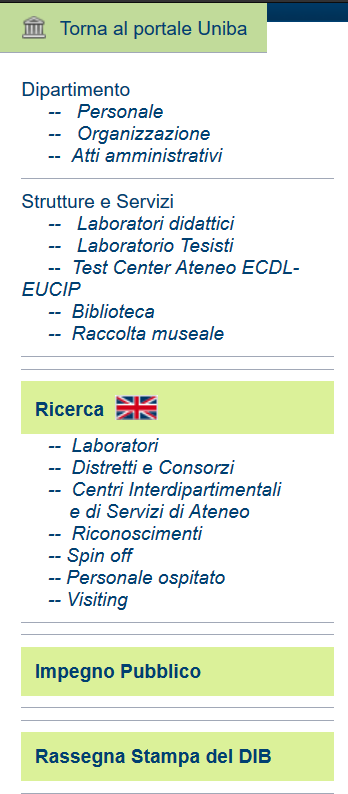
\includegraphics[width=.7\linewidth]{C:/Users/elepo/Desktop/UNI/WIM/ANALISI_SITO/Relazione/sez/Analisi/311.png}
     \caption{Parte sinistra 1}
   \end{minipage}\hfill
   \begin{minipage}{0.48\textwidth}
     \centering
     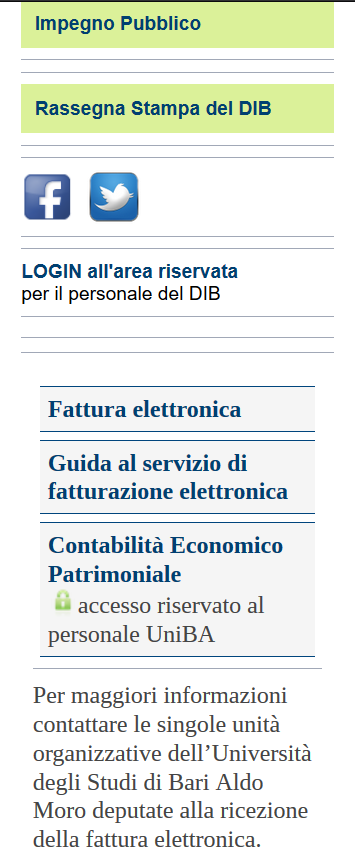
\includegraphics[width=.7\linewidth]{C:/Users/elepo/Desktop/UNI/WIM/ANALISI_SITO/Relazione/sez/Analisi/312.png}
     \caption{Parte sinistra 2}
   \end{minipage}
\end{figure}	
		
		
		
		
		
		
		
		
		

\newpage
				\item Parte centrale: nella parte superiore troviamo informazioni generali sul dipartimento (indirizzo, direttore, coordinatore) mentre nella parte sottostante diverse sezioni dedicate a eventi, news
				\begin{center}
\begin{figure}[h!]
           \begin{center}
           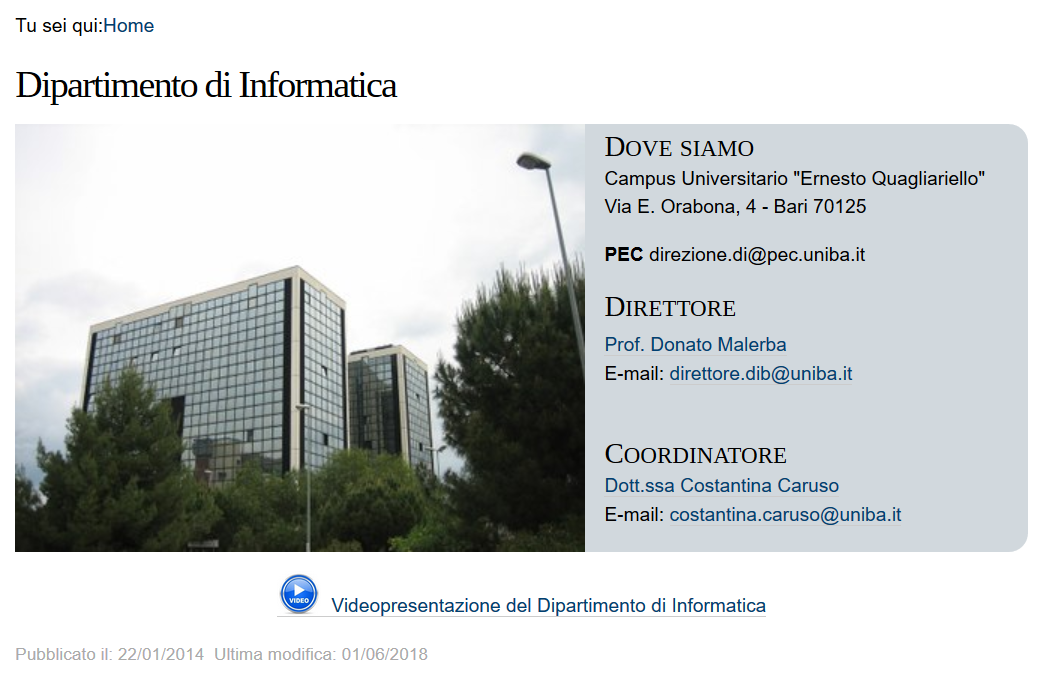
\includegraphics[scale=0.40]{C:/Users/elepo/Desktop/UNI/WIM/ANALISI_SITO/Relazione/sez/Analisi/321.png}
           \caption{Parte centrale 1}
           \end{center}
  \end{figure}
\end{center}
\begin{center}
\begin{figure}[h!]
           \begin{center}
           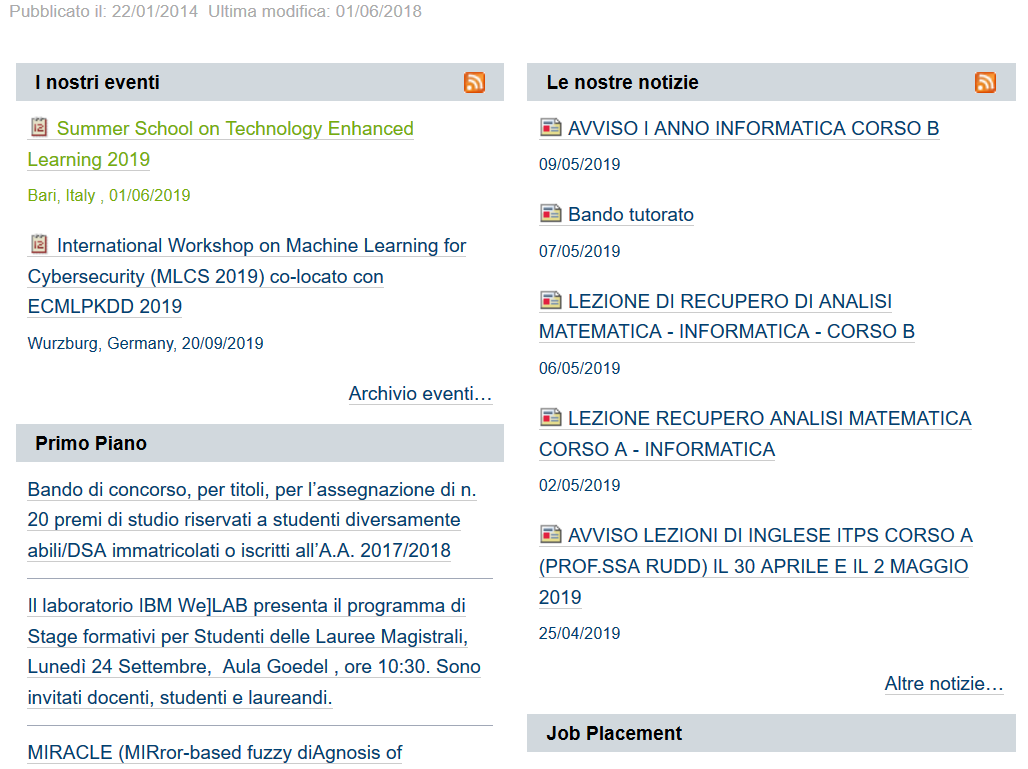
\includegraphics[scale=0.40]{C:/Users/elepo/Desktop/UNI/WIM/ANALISI_SITO/Relazione/sez/Analisi/322.png}
           \caption{Parte centrale 2}
           \end{center}
  \end{figure}
\end{center}
\newpage
				\item Parte destra: riservata alle sezioni del sito in lingua inglese, didattica, due sezioni per master, portale di login per gli studenti della facoltà, informazioni generali sulla segreteria didattica
\begin{figure}[!htb]
   \begin{minipage}{0.48\textwidth}
     \centering
     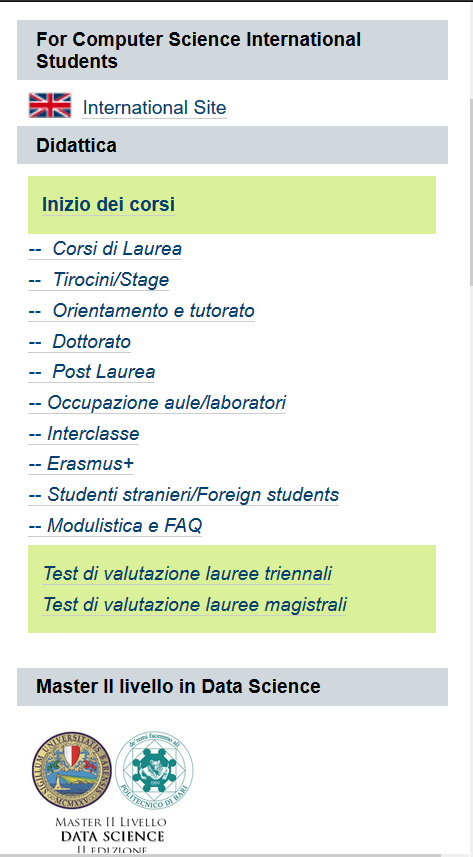
\includegraphics[width=.7\linewidth]{C:/Users/elepo/Desktop/UNI/WIM/ANALISI_SITO/Relazione/sez/Analisi/331.png}
     \caption{Parte destra 1}
   \end{minipage}\hfill
   \begin{minipage}{0.48\textwidth}
     \centering
     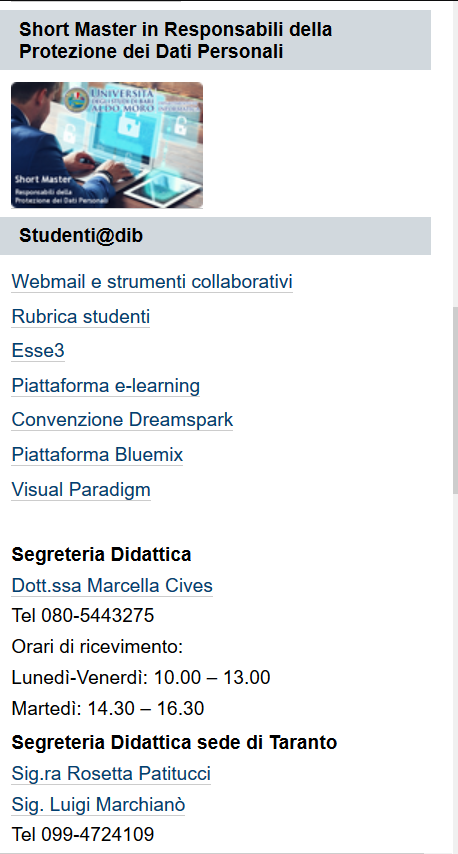
\includegraphics[width=.7\linewidth]{C:/Users/elepo/Desktop/UNI/WIM/ANALISI_SITO/Relazione/sez/Analisi/332.png}
     \caption{Parte destra 2}
   \end{minipage}
\end{figure}					
				
				
				
				
			
			\end{itemize}
		\item \textbf{Footer}: si colloca nella parte inferiore della pagina e contiene contatto con i social (di nuovo), sezioni di diversa natura e le solite informazioni contenute in questa sezione.
		\begin{center}
\begin{figure}[h!]
           \begin{center}
           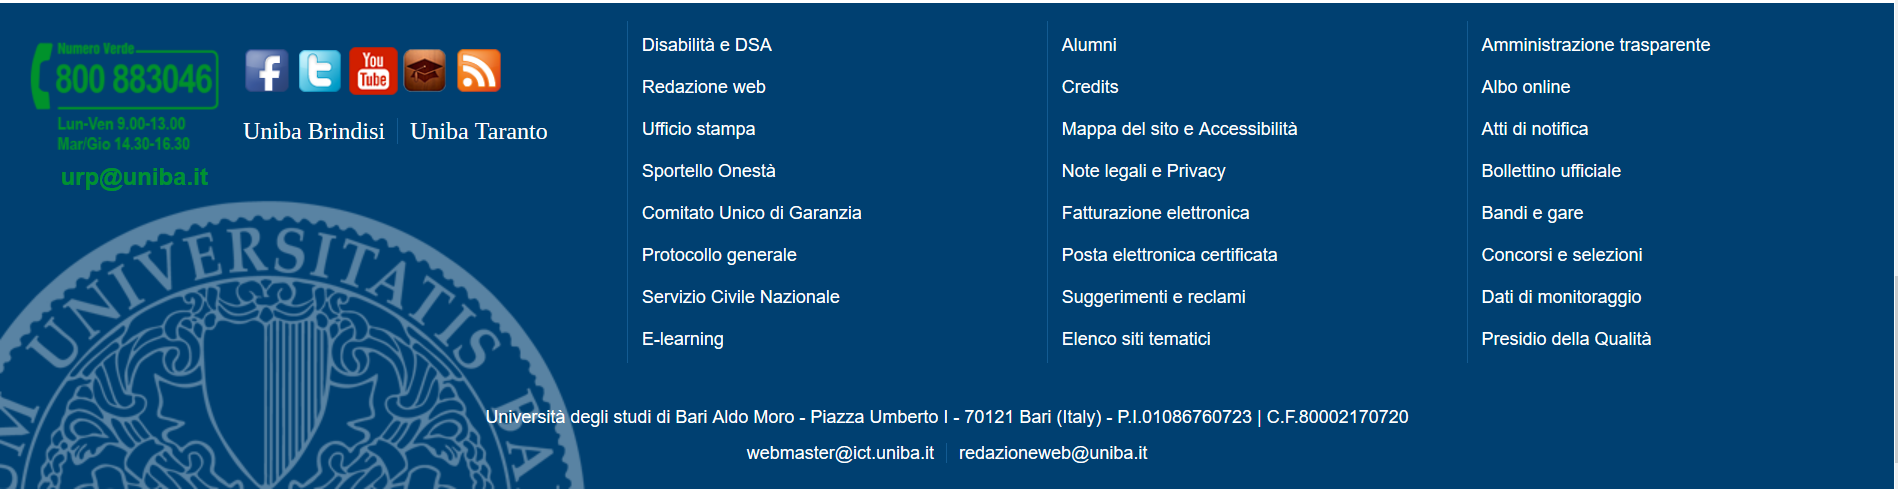
\includegraphics[scale=0.40]{C:/Users/elepo/Desktop/UNI/WIM/ANALISI_SITO/Relazione/sez/Analisi/4.png}
           \caption{Footer}
           \end{center}
  \end{figure}
\end{center}
			
	\end{itemize}
\newpage




Il sito analizzato fa parte della pagina web dedicata all'Ateneo dell'università di Bari. \\
Arrivati alla homepage del sito dedicato al Dipartimento di Informatica esistono sottosezioni dedicate per soddisfare diverse esigenze.
Le principali sottosezioni che si individuano sono le seguenti:
	\begin{itemize}
		\item \textbf{Dipartimento}: contiene informazioni sul personale, organizzazione del dipartimento (consiglio, giunta, coordinatore..) e 		lo storico dell'attività amministrativa;
		\item \textbf{Strutture e servizi}: all'interno della quale sono elencate le infrastrutture (per esempio laboratori);
		\item \textbf{Ricerca}: dove troviamo tutte le informazioni relative all'attività di ricerca del Dipartimento;
		\item \textbf{Impegno pubblico}: dove sono esposte le iniziative di carattere culturale e sociale del Dipartimento;
		\item \textbf{Rassegna stampa del dipartimento};
		\item \textbf{Didattica}: dove compaiono tutte le informazioni riguardanti il corso di studi;
		\item \textbf{I nostri eventi};
		\item \textbf{Primo piano};
		\item \textbf{Le nostre notizie};
		\item \textbf{Job placement};
		\item \textbf{Master II livello in Data Science};
		\item \textbf{Short Master in Responsabili della Protezione dei Dati Personali};
		\item \textbf{Studenti@dib};
		\item \textbf{For Computer Science International Students}: sito in versione inglese.
	\end{itemize}
La strutturazione delle sezioni è molto caotica: vengono utilizzati diversi pattern visivi per sottosezioni che logicamente sembrerebbero essere della stessa entità, creando confusione nell'utente in merito alla gerarchia delle sezioni.\\
Sono stati individuati 4 tipi di pattern differenti:
	\begin{itemize}
		\item \textbf{Testo semplice blu}: vedi sezione "Dipartimento", "Strutture e servizi";
		
		\item \textbf{Testo blu grassetto su sfondo verde}: per le sezioni "Ricerca" (affiancata da una bandiera inglese di cui non si capisce 						  il senso), "Impegno pubblico", "Rassegna stampa", 
		\item \textbf{Testo blu grassetto sottolineato in grigio su sfondo verde}: si trova nella sotto-sezione "Inizio dei corsi";
		\item \textbf{Testo blu corsivo sottolineato in grigio su sfondo verde}: si trova nelle sotto-sezioni riguardanti i test di 								  valutazione;
		\item \textbf{Testo nero grassetto su sfondo grigio}: per la sezione "Didattica", "Primo piano", "I nostri eventi", "Le nostre 								  notizie", "Job placement", "Studenti @dib", "Short Master in responsabili della protezione dei dati personali"; "Master 						  in data science", "For Computer Science International Students". Inoltre in queste sezioni esiste ancora più incongruenza, dal momento che alcune di queste sono cliccabili ("Le nostre notizie", "in primo piano", "i nostri eventi") con testo che diventa verde quando ci si passa sopra con il cursore, altre non sono cliccabili ma contengono sottosezioni riportate sotto forma di elenchi cliccabili e altre ancora non hanno sottosezioni riportate sotto forma di elenco, ma hanno delle immagini cliccabili che riportano al sito dedicato ("Master II livello in Data Science" e "Short Master in Responsabili della Protezione dei Dati Personali").
	\end{itemize}
Inoltre esistono anche tre pattern differenti per indicare le sottosezioni incluse nelle sezioni precedentemente elencate:
	\begin{itemize}
		\item \textbf{Testo corsivo blu preceduto da doppi trattini}: per gli elenchi appartenenti alle sezioni "Dipartimento", "Strutture e servizi" e "ricerca". Quando si passa sul cursore sul testo non accade nulla;
		\item \textbf{Testo corsivo blu sottolineato grigio preceduto da doppi trattini}: per gli elenchi appartenenti alla sezione "Didattica". Quando si passa sul cursore sul testo diventa verde;
		\item \textbf{Testo corsivo blu sottolineato grigio senza trattini}: per gli elenchi appartenenti alla sezione "Studenti @dib". Quando si passa sul cursore sul testo diventa verde.
	\end{itemize}

In linea teorica è corretto utilizzare pattern differenti per esibire sezioni di diversa importanza, ma bisogna fare attenzione nell'usare questa tecnica onde evitare di impedire all'utente di fare uno scanning corretto del sito. \\
Nel sito in esame il risultato è disastroso: si privilegiano e mettono in primo piano contenuti di importanza secondaria (vedi sezione "Rassegna stampa del Dib") e le sezioni di uguale importanza (per esempio "Didattica" e "Strutture e servizi", entrambi di carattere informativo in merito alle strutture e alle opportunità offerte dall'ateneo) sono evidenziate con pattern differenti.\\
Inoltre vi è un senso di incongruenza generale che peggiora ancora di più l'impatto visuale, come se le diverse sezioni fossero state incollate tra di loro senza un minimo di criterio.\\
Un altro aspetto negativo consiste nel fatto che le diverse sezioni non sono organizzate all'interno di un menù che le contenga tutte, ma sono distribuite in maniera del tutto casuale all'interno della pagina (a sinistra, a destra, nella parte centrale). Vi è una forte dispersione.\\
Infine va sottolineato che il menù in alto a destra nella pagina non è relativo al sito del dipartimento di informatica, ma all'ateneo UniBa, quindi in questa analisi non verrà citato. Si sottolinea solamente che non è scontato supporre che l'utente sappia che le voci del menù in alto reindirizzano al sito UniBa, e questo potrebbe scaturire confusione.



